%
% LaTeX template for the XLVI CILAMCE
%
\documentclass[a4paper,10pt]{book}

% PACKAGES USED - packages that need to be previously installed on your computer
\usepackage[lmargin=2.5cm, rmargin=2.5cm, tmargin=2.5cm, bmargin=2.5cm ]{geometry}
\usepackage{graphicx}
\usepackage{times}
\usepackage{indentfirst}
\usepackage{fancyhdr}
\usepackage{titlesec}
\usepackage[english]{babel}
\usepackage{parskip} 
\usepackage{setspace}


%Package to hold figure in position
\usepackage{placeins}


% Mathematical Symbols
\newcommand{\dgds}{\boldsymbol{g_\sigma}}
\newcommand{\Dll}{\boldsymbol{D}}
\newcommand{\Dllmod}{\boldsymbol{D^{*}}}
\newcommand{\Dllepvp}{\boldsymbol{D}^{epvp}}
\newcommand{\dstrain}{\boldsymbol{\dot{\varepsilon}}}
\newcommand{\dstraine}{\boldsymbol{\dot{\varepsilon}}^{e}}
\newcommand{\dstrainp}{\boldsymbol{\dot{\varepsilon}}^{p}}
\newcommand{\dstrainv}{\boldsymbol{\dot{\varepsilon}}^{vp}}
\newcommand{\straineqp}{\bar \varepsilon^p}
\newcommand{\dstrainsh}{\boldsymbol{\dot{\varepsilon}}^{sh}}
\newcommand{\dstraincr}{\boldsymbol{\dot{\varepsilon}}^{cr}}
\newcommand{\dstress}{\boldsymbol{\dot{\sigma}}}

\newcommand{\ex}{\boldsymbol{e}_x}
\newcommand{\ey}{\boldsymbol{e}_y}
\newcommand{\ez}{\boldsymbol{e}_z}

\newcommand{\onell}{\boldsymbol{1}}
\newcommand{\strain}{\boldsymbol{\varepsilon}}
\newcommand{\straincr}{\boldsymbol{\varepsilon}^{cr}}
\newcommand{\straine}{\boldsymbol{\varepsilon}^{e}}
\newcommand{\strainp}{\boldsymbol{\varepsilon}^{p}}
\newcommand{\strainsh}{\boldsymbol{\varepsilon}^{sh}}
\newcommand{\strainshCEB}{\varepsilon_{sh}}
\newcommand{\strainvp}{\boldsymbol{\varepsilon}^{vp}}
\newcommand{\stress}{\boldsymbol{\sigma}}
\newcommand{\zerol}{\boldsymbol 0}



%%%%%%%%%%%%%%%%%%%%%%%%%%%%%%%%%%%%%%%%%%%%%%%%%%%%%%%%%%%%%%%%%
%%%%%%%%%%%%%%%%%%%%%%%%%%%%%%%%%%%%%%%%%%%%%%%%%%%%%%%%%%%%%%%%%
%%% My Additional Packages
%%%%%%%%%%%%%%%%%%%%%%%%%%%%%%%%%%%%%%%%%%%%%%%%%%%%%%%%%%%%%%%%%
\usepackage[utf8]{inputenc}
\usepackage{amssymb} %Mathematics
\usepackage{amsfonts}%Mathematics
\usepackage{amsmath,amscd}%Mathematics
\usepackage{amsthm}%Mathematics
\usepackage{mathrsfs}%Mathematics font
\usepackage{xspace}
\usepackage{booktabs}
\usepackage{stmaryrd}%Particular Brackets
\usepackage{graphicx} %Tables and Figures
\usepackage{subfigure}
\usepackage{url}
\usepackage{hyperref}
\usepackage{cleveref}
\usepackage{./pkg-crefNames}
\usepackage[labelsep=period]{caption}
%\usepackage{mathptmx}
\usepackage{newtxtext,newtxmath}
\usepackage{bm}

\hypersetup{hidelinks}

%\usepackage[utf8]{inputenc}
%%\usepackage{amssymb} %Mathematics
%%\usepackage{amsfonts}%Mathematics
%\usepackage{amsmath,amscd}%Mathematics
%%\usepackage{amsthm}%Mathematics
%%\usepackage{mathrsfs}%Mathematics font
%%\usepackage{xspace}
%%\usepackage{booktabs}
%%\usepackage{stmaryrd}%Particular Brackets
%%\usepackage{graphicx} %Tables and Figures
%%\usepackage{subfigure}
%%\usepackage{url}
%\usepackage{hyperref}
%\usepackage{cleveref}
%\usepackage{./pkg-crefNames}
%\usepackage[labelsep=period]{caption}
\usepackage{makecell}

%BibTeX compatible with the CILAMCE format
\usepackage[numbers,sort&compress]{natbib}

\setlength{\bibsep}{0pt plus 0.3ex}

\renewcommand*{\bibfont}{\small}

\makeatletter
\renewcommand\bibsection
{
  \section*{References}
}

\renewenvironment{thebibliography}[1]
      {\section*{\refname}%
       \@mkboth{\MakeUppercase\refname}{\MakeUppercase\refname}%
       \list{\@biblabel{\@arabic\c@enumiv}}%
            {\settowidth\labelwidth{\@biblabel{#1}}%
             \leftmargin\labelwidth
             \advance\leftmargin-10pt% change 20 pt according to your needs
             \advance\leftmargin\labelsep
             \setlength\itemindent{10pt}% change using the inverse of the length used before
             \@openbib@code
             \usecounter{enumiv}%
             \let\p@enumiv\@empty
             \renewcommand\theenumiv{\@arabic\c@enumiv}}%
       \sloppy
       \clubpenalty4000
       \@clubpenalty \clubpenalty
       \widowpenalty4000%
       \sfcode`\.\@m}
      {\def\@noitemerr
        {\@latex@warning{Empty `thebibliography' environment}}%
       \endlist}
\renewcommand\newblock{\hskip .11em\@plus.33em\@minus.07em}
\makeatother

\makeatother
\bibliographystyle{./bib-cilamce}
%\bibliographystyle{plain}

%%%%%%%%%%%%%%%%%%%%%%%%%%%%%%%%%%%%%%%%%%%%%%%%%%%%%%%%%%%%%%%%%
%%%%%%%%%%%%%%%%%%%%%%%%%%%%%%%%%%%%%%%%%%%%%%%%%%%%%%%%%%%%%%%%%

% CONFIGURATION
\renewcommand*\arraystretch{1.5}
\renewcommand*\thesection{\arabic{section}}
%\hyphenpenalty=10000 % You can uncomment this to avoid hyphenization
\titleformat*{\section}{\large\bfseries}
\titleformat*{\subsection}{\bfseries}
\titlespacing\section{0pt}{20pt plus 2pt minus 2pt}{12pt plus 2pt minus 2pt}
\titlespacing\subsection{0pt}{20pt plus 0pt minus 0pt}{12pt plus 0pt minus 0pt}
\setlength{\parskip}{0pt} % Spacing between paragraphs
\setlength{\parindent}{0.75cm} % Paragraph identation
\setlength\abovecaptionskip{6pt}

% --------------------------------------------------------------------------
% DO NOT EDIT - SPECIAL HEADINGS OF XLIII CILAMCE
% --------------------------------------------------------------------------
\fancypagestyle{first}
{
\fancyhf{}
\fancyfoot[RO]{\footnotesize \textit{CILAMCE-2025 \\
Proceedings of the XLVI Ibero-Latin-American Congress on Computational Methods in Engineering, ABMEC\\
Vitória, Brazil, November 24-27, 2025}}
\renewcommand{\headrulewidth}{.0pt}
\renewcommand{\footrulewidth}{.5pt}
}

\pagestyle{fancy}
\fancyhf{}

\fancyfoot[LE]{\footnotesize \textit{CILAMCE-2025\\
Proceedings of the XLVI Ibero-Latin-American Congress on Computational Methods in Engineering, ABMEC\\
Vitória, Brazil, November 24-27, 2025}}

\fancyfoot[RO]{\footnotesize \textit{CILAMCE-2025\\
Proceedings of the XLVI Ibero-Latin-American Congress on Computational Methods in Engineering, ABMEC\\
Vitória, Brazil, November 24-27, 2025}}

\renewcommand{\headrulewidth}{.5pt}
\renewcommand{\footrulewidth}{.5pt}

% --------------------------------------------------------------------------
% PLEASE, EDIT THIS!
\fancyhead[LE]{\footnotesize \textit{Numerical analysis of deformations in deep twin tunnels with a transverse gallery}}
\fancyhead[RO]{\footnotesize \textit{Bianca M. Girardi, Felipe P. M. Quevedo, Samir Maghous}}
% --------------------------------------------------------------------------

\begin{document}\thispagestyle{first}

% --------------------------------------------------------------------------
% DO NOT EDIT - LOGO OF XLIII CILAMCE
% --------------------------------------------------------------------------

\begin{figure}[ht!]
\vspace{-30pt}
\flushright
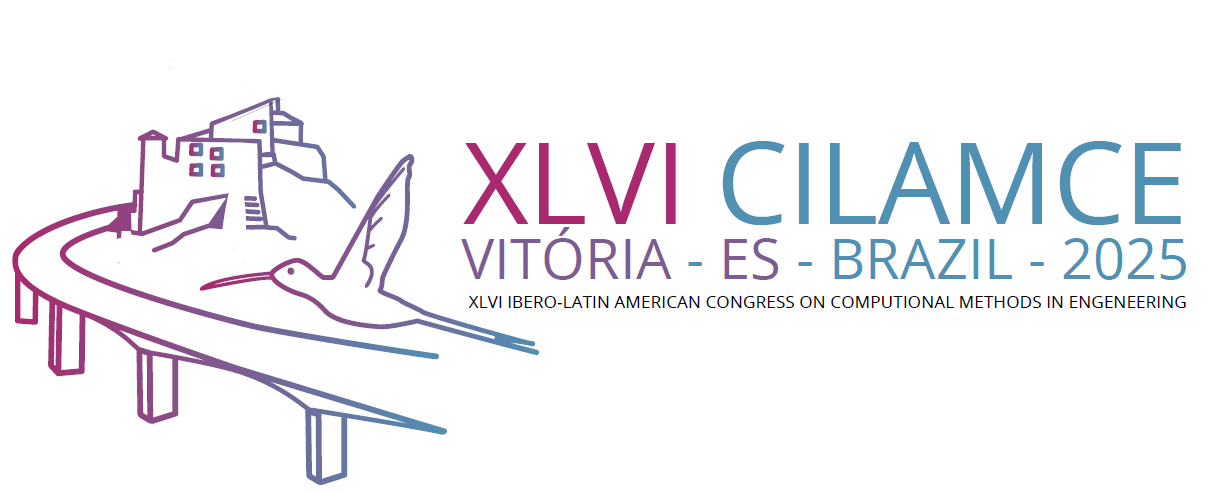
\includegraphics[width=6.69cm]{Figures/logo.png}
%scale=0.25
\end{figure}

% --------------------------------------------------------------------------
% TITLE OF PAPER
% --------------------------------------------------------------------------

\noindent
\textbf{\Large
Pressure anisotropy on twin tunnel linings induced by a transverse gallery construction using time-dependent constitutive models} 
\vspace{18pt} % <- keep this vertical space!

% --------------------------------------------------------------------------
% AUTHORS
% --------------------------------------------------------------------------

\noindent Bianca M. Girardi$^1$, Felipe P. M. Quevedo$^1$, Samir Maghous$^1$

\vspace{18pt} % <- keep this vertical space!

\noindent $^1$\textit{Graduate Program in Civil Engineering, Federal University of Rio Grande do Sul}

\noindent \textit{Av. Osvaldo Aranha, 99, Porto Alegre, 90.035-190, RS, Brazil}

\noindent \textit{eng.biancagirardi@gmail.com, motta.quevedo@ufrgs.br, samir.maghous@ufrgs.br}

%\noindent $^2$\textit{Dept. of Something Else, University of Somewhere Else}

%\noindent \textit{Address, Zip-Code, State/Province, Country}

%\noindent \textit{somebody3@somewhere.com}


\vspace{18pt} % <- keep this vertical space!

% --------------------------------------------------------------------------
% ABSTRACT
% --------------------------------------------------------------------------

\noindent \textbf{Abstract.} The increasing construction of twin tunnels demands a comprehensive understanding of their interaction with transverse galleries and the surrounding rock mass. This study conducts a 3D finite element analysis of the junction between deep twin tunnels and a transverse gallery, incorporating time-dependent effects such as rock mass creep, concrete creep, and shrinkage. The model is verified against existing numerical results, confirming its reliability in estimating internal forces in the lining. The influence of different rock mass friction angles on pressure distributions is investigated, revealing that higher friction angles significantly reduce lining pressures, particularly at the end of tunnel construction. The results indicate pronounced anisotropy in pressures, influenced by the properties of the lining and the rock mass, and peak pressures are observed at the lateral sides of the walls. Additionally, viscoelastic linings exhibit increased long-term stress redistribution, emphasizing the role of rheological behavior in tunnel performance. These findings offer valuable insights for the design and reinforcement of tunnel–gallery intersections. The study reinforces the importance of 3D modeling and time-dependent behavior in the safe and accurate design of tunnel–gallery intersections.


%The increasing construction of twin tunnels demands a comprehensive understanding of their interaction with transverse galleries and the surrounding rock mass. This study conducts a 3D finite element analysis of the junction between deep twin tunnels and a transverse gallery, incorporating time-dependent effects such as rock mass creep, concrete creep, and shrinkage. The model is verified against existing numerical results, confirming its reliability in estimating internal forces in the lining. A comparison of different rock mass friction angles demonstrates their impact on pressure distributions along the lining, providing relevant insights for design and reinforcement strategies. The results indicate pronounced anisotropy in pressures, influenced by the properties of the lining and the rock mass, and peak pressures are observed at the lateral sides of the walls. A higher friction angle contributes to pressure reduction, especially at the end of tunnel construction. Viscoelastic linings show increased long-term redistribution of stresses. The study reinforces the importance of 3D modeling and time-dependent behavior in the safe and accurate design of tunnel–gallery intersections.


\vspace{18pt} % <- keep this vertical space!

\noindent \textbf{Keywords:} Deep twin tunnels, Transverse gallery, Viscoelastic concrete lining, Elastoplastic-viscoplastic coupled, Finite element model


% --------------------------------------------------------------------------
\section{Introduction}\label{sec:introduction}
% --------------------------------------------------------------------------
The increasing demand for underground infrastructure in urban areas has led to a rise in the construction of twin tunnels, typically designed for one-way traffic in each tunnel. For operational and safety purposes, transverse galleries are often incorporated, allowing for interconnections between tunnels. These junction zones represent critical areas in tunnel design due to the complex interactions between the tunnel linings, surrounding rock mass, and construction sequence.

Despite advances in tunneling technology, the interaction mechanisms induced by transverse galleries, especially in deep tunneling scenarios, remain underexplored, mainly due to the computational complexity involved in modeling 3D geometries and sequential excavation processes. The excavation of a transverse gallery causes a redistribution of stresses in the surrounding rock mass, resulting in increased loads on the main tunnel lining near the intersection. When these additional loads exceed the structural capacity of the primary lining, localized instability may occur, raising the risk of failure. Therefore, understanding how deformations and pressures are redistributed in this zone is crucial for the proper design of linings and the placement of structural reinforcements. Incorporating these effects into the design process is essential to ensure the structural integrity and long-term stability of the tunnel system.

The present work extends a previous numerical study by \citet{Quevedoetal2025}, providing a detailed three-dimensional finite element analysis of deep twin tunnels connected by a transverse gallery. A coupled elastoplastic-viscoplastic constitutive model is used for the rock mass, while the concrete lining behavior includes viscoelasticity and shrinkage effects. Special attention is given to the anisotropic redistribution of lining pressures in the junction zone, considering different friction angles in the rock mass and comparing elastic and viscoelastic linings.

The results aim to support design decisions by highlighting the importance of using advanced material models and 3D simulations in the analysis of tunnel-gallery intersections, particularly under long-term conditions.

% --------------------------------------------------------------------------
\section{Constitutive models}\label{sec:format}
% --------------------------------------------------------------------------

The structural response of the tunnel system is governed by time-dependent behaviors in both the concrete lining and the surrounding rock mass. 


% --------------------------------------------------------------------------
\subsection{Concrete lining} \label{constitmodelconcrete}
% --------------------------------------------------------------------------

The viscoelastic behavior of concrete is modeled using the Solidification Theory developed by \citet{BazantPrasannanA,BazantPrasannanB}, calibrated with the CEB-FIP Model Code 1990 standard specifications formulation described
in \citet{CEB1993}. This formulation enables the simulation of delayed deformations and stress redistribution caused by creep and shrinkage in the lining. The creep strain is represented through a Generalized Kelvin chain with aging, while shrinkage is introduced as an isotropic strain field. The stress–strain relationship under small deformations is expressed as:
\begin{center}
	\begin{equation}
		\Delta \stress = \Dll : \Delta \strain - \Dll : \Delta \strainsh - \Dllmod : \Delta \straincr
		\label{Eq1}
	\end{equation}
\end{center}
where $\Dll$ is the elastic constitutive tensor, $\Dllmod$ is the same tensor reformulated to account for the viscoelastic effects due to concrete aging, and $\Delta \strainsh$ and $\straincr$ are the shrinkage and creep strain increments, respectively.

To match the CEB-FIP MC90 formulation, the parameters of the Bažant-Prasannan model are calibrated through the following equivalences:
\begin{center}
	\begin{equation}
		E_0 = E_c(t_0), \quad \gamma(t - t_0) = \beta_c(t - t_0), \quad \dfrac{1}{v(t)} = \dfrac{\varphi_0(t_0)}{E_{ci}}, \quad \dfrac{1}{\eta(t)} \rightarrow 0
		\label{Eq2}
	\end{equation}
\end{center}

In Equation (\ref{Eq2}), $t_0$ represents the concrete age at the time of loading; $E_c(t_0)$ is the tangent modulus at loading; $\beta_c(t-t_0)$ is a function of the age of loading; $\varphi_0(t_0)$ is the basic creep coefficient; $E_{ci}$ is the elastic modulus at 28 days; and $\eta(t)$ is the apparent macroscopic viscosity.

% --------------------------------------------------------------------------
\subsection{Rock mass} \label{constitmodelrockmass}
% --------------------------------------------------------------------------

The rock mass is modeled using a coupled elastoplastic-viscoplastic formulation under infinitesimal strain theory. The total strain rate $\dstrain$ is decomposed into elastic $\dstraine$, plastic $\dstrainp$, and viscoplastic $\dstrainv$ components:
\begin{center}
	\begin{equation}
		\dot{\boldsymbol{\varepsilon}} = \dot{\boldsymbol{\varepsilon}}^{e} + \dot{\boldsymbol{\varepsilon}}^{p} + \dot{\boldsymbol{\varepsilon}}^{vp}
		\label{Eq3}
	\end{equation}
\end{center}
where:
\begin{equation}
	\dstrainp = \begin{cases} 
		\dot{\lambda}^p \dfrac{\partial f^p}{\partial \stress}, & \text{for } f^p > 0, \\ 
		\boldsymbol{0}, & \text{for } f^p \le 0,
	\end{cases}
 	, \quad \text{and } \quad \dstrainv = \dfrac{\langle f^{vp}\rangle^n}{\eta} \dfrac{\partial f^{vp}}{\partial \stress}
	\label{Eq6}
\end{equation}
where $\dot{\lambda}^p$ and $\dot{\lambda}^p$ denotes, respectively, the plastic and viscoplastic multiplier, $f^p$ and $f^{vp}$ is the plastic and viscoplastic yield function, $\eta$ is the dynamic viscosity constant (in MPa.day), $n$ is the dimensionless parameter and $\langle \ast \rangle$ is the McCauley function. The short-term behavior is captured using the Drucker–Prager yield criterion:
\begin{center}
	\begin{equation}
		f^p(\boldsymbol{{\sigma}},q) = f^p(I_1, J_2, q^p)= \beta_1 I_1 + \beta_2 \sqrt{J_2} - q^p(\alpha^p).
		\label{Eq4}
	\end{equation}
\end{center}
The yield surface is defined in terms of the first invariant of stress tensor $I_1$, the second invariant of the deviator tensor $J_2$, the parameter related to cohesion $q^p(\alpha^p)$ and the strength parameters related to the friction angle $\beta_1$ and $\beta_2$. These terms are given by:
\begin{center}
	\begin{equation}
		\beta_1 = \dfrac{(k^p-1)}{3}, \beta_2 = \dfrac{(2k^p+1)}{\sqrt{3}}, q^p(\alpha^p)= 2\sqrt{k^p}c^p(\alpha^p),
		\label{Eq5}
	\end{equation}
\end{center}
\noindent where $k^p = (1+\sin{\phi^p})/(1-\sin{\phi^p})$ and $\alpha^p$ is the internal variable associated with the hardening and softening of the material.

Consistent with the elastoplastic approach, the viscoplastic yield function also adopts the Drucker–Prager yield criterion. As a consequence, the coefficients $\beta_1$ and $\beta_2$ of eq. (\ref{Eq5}) are evaluated by replacing $k^p$ for $k^{vp} = (1+\sin{\phi^{vp}})/(1-\sin{\phi^{vp}})$. Also, the viscoplastic cohesion parameter then becomes $q^{vp} = 2\sqrt{k^{vp}}c^{vp}(\alpha^{vp})$. In this study, both plastic and viscous flow rules are implemented with associative potentials, assuming perfect plasticity and viscoplasticity (i. e., cohesions $c^p$ and $c^{vp}$ assumed to remain constant).

% --------------------------------------------------------------------------
\section{Spatial and time discretization of the domain}\label{sec:domain}
% --------------------------------------------------------------------------

The finite element simulations were performed using a three-dimensional model representing deep twin tunnels connected by a transverse gallery. The geometry was reduced by symmetry, modeling only one-quarter of the domain, represented as $\Omega$ (see \cref{Fig1}). The analysis assumes deep tunnel conditions ($H \gg R_t$), with $H$ being the overburden depth and $R_t$ the longitudinal tunnel radius. The transverse gallery radius $R_g$ is smaller than $R_t$ ($R_g < R_t$).

\begin{figure}[!ht]
	\begin{center}
		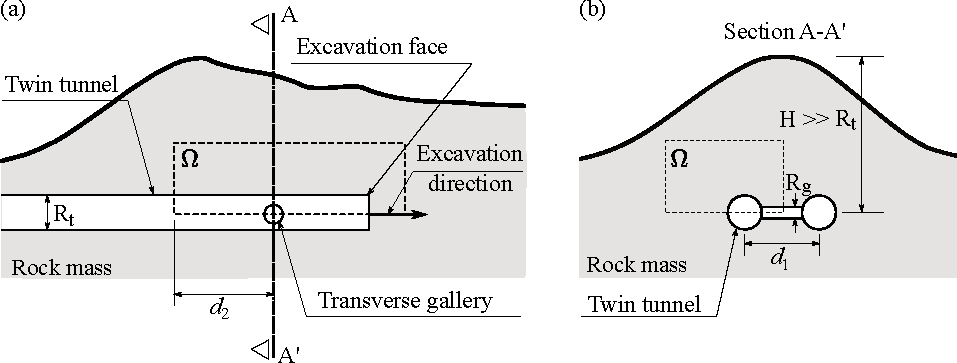
\includegraphics[scale=0.8]{Figures/Fig1.pdf}
		\vspace{12pt}
		\caption{Schematic representation of the twin tunnels geometry problem: (a) longitudinal view and (b) section A-A’.}
		\label{Fig1}
	\end{center}
\end{figure}

The computational domain consists of a parallelepiped volume with dimensions $(L_1 + L_2) \times L_3 \times d_3$, as presented in \cref{Fig2}. Symmetry conditions are imposed on the planes $ x = 0 $, $ y = 0 $, and $ z = L_1+L_2 $, reducing the computational cost of the analysis. This approach assumes that the longitudinal tunnels are excavated synchronously and the transverse gallery is excavated from the tunnels towards the center. Initial isotropic in-situ stresses are applied as boundary pressures: vertical stress $\sigma_v$ at the upper plane and horizontal stress $\sigma_h$ at the left-lateral and back planes.

Discretization is performed using 8-node trilinear hexahedral elements with full integration. In regions with complex geometry, such as the tunnel-gallery intersection, 8-node linear tetrahedral elements are used. A refined mesh is employed in the zones near the tunnel and gallery walls to ensure accuracy in stress and deformation fields. The total mesh consists of approximately 617,000 elements.

The geometric and construction parameters adopted in the analysis define the radius of the longitudinal tunnels as $R_t$, while the radius of the gallery is set to $R_g = 0.5R_t$. The thickness of the concrete lining is the same for both the longitudinal tunnels and the gallery, given by $e_t=e_g=0.05R_t$. Also, the distance between longitudinal tunnel axes is denoted by $d_1=4R_t$.

The excavation process is modeled using an activation–deactivation technique. The longitudinal tunnel excavation is simulated by deactivating solid elements (reducing their stiffness), followed by activation of lining elements after a specified distance from the face ($d_{0t}=2R_t/3$). Each excavation step ($L_{pt}=R_t/3$) is associated with a time interval $t_p = L_{pt}/V_{pt}$, where $V_{pt} = 12.5$ m/day is the excavation speed. The gallery is excavated after complete a predefined number of steps ($n_{pig}$) in the longitudinal tunnel and follows the same procedure with $L_{pg}=0.2R_g$, $V_{pg}=12.5$ m/day and $d_{0g}$.

\begin{figure}[!h]
	\begin{center}
		\includegraphics[scale=0.07]{Figures/Fig2.pdf}
		\vspace{12pt}
		\caption{Mesh, dimensions and boundary conditions of the twin tunnels with gallery domain.}
		\label{Fig2}
	\end{center}
\end{figure}
%\FloatBarrier

\begin{figure}[!ht]
	\begin{center}
		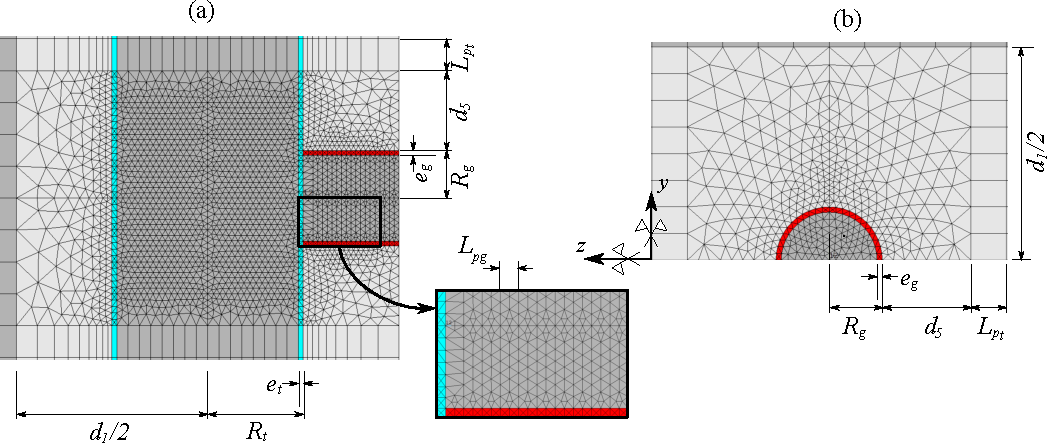
\includegraphics[scale=0.75]{Figures/Fig3.pdf}
		\vspace{12pt}
		\caption{Geometry and F. E mesh: (a) longitudinal tunnel and gallery in the symmetry plane y = 0 and (b) gallery cross-section}
		\label{Fig3}
	\end{center}
\end{figure}
%\FloatBarrier

%Material ages and durations are tracked in time steps consistent with the construction sequence to ensure correct application of time-dependent behavior. This approach allows the numerical model to capture the interaction between excavation-induced stress redistribution and the long-term mechanical response of both the rock mass and the lining. 

%\vspace{8pt}
%\begin{table}[!ht]
%	\centering
%	\caption{Geometric and construction parameters of the domain}
%	\label{Table1}
%	\vspace{0pt}
%	\begin{tabular}{cccc}
%		\hline
%		Parameters & Symbol & Unit & Value \\[-2pt] \hline
%		\multicolumn{4}{c}{Longitudinal tunnels} \\ [-2pt] \hline
%		Radius & $R_t$ & m & $R_t$ \\[-3pt]
%		Thickness of the concrete lining & $e_t$ & m & $0.05R_t$ \\[-3pt]
%		Step length of the excavation process & $L_{pt}$ & m & $R_t/3$ \\[-3pt]
%		Unlined length & $d_{0t}$ & m & $2R_t/3$ \\[-3pt] \hline
%		\multicolumn{4}{c}{Gallery} \\ [-2pt] \hline
%		Radius & $R_g$ & m & $0.5R_t$ \\[-3pt]
%		Thickness of the concrete lining & $e_g$ & m & $0.05R_t$ \\[-3pt]
%		Step length of the excavation process & $L_{pg}$ & m & $0.2R_g$ \\[-3pt]
%		Unlined length & $d_{0g}$ & m & $0$ \\[-3pt]
%		Steps before gallery excavation & $n_{pig}$ & un & $15$ \\[-3pt] \hline
%		%\multicolumn{4}{c}{Rest of domain} \\ [-2pt] \hline
%		%Distance between longitudinal tunnel axes & $d_1$ & m & $4R_t$ \\[-3pt]
%		%Thickness along vertical direction $\mathbf{e}_y$ & $d_3$ & m & $20R_t$ \\[-3pt]
%		%\makecell[c]{Distance of transition zone between tetrahedral \\ and hexahedral elements} & $d_5$ & m & $2L_p$ \\[-3pt]
%		%Length of the unexcavated region & $L_1$ & m & $10R_t$ \\[-3pt]
%		%Total excavated length & $L_2$ & m & $500L_{pt}$ \\[-3pt]
%		%Thickness along transversal direction $\mathbf{e}_z$ & $L_3$ & m & $20R_t + d_1/2$ \\[-3pt] \hline
%	\end{tabular}
%\end{table}
%\FloatBarrier
%\vspace{8pt}

%\begin{table}[h!]
%	\centering
%	\caption{Geometric and construction parameters of the domain}
%	\label{Table1}
%	\vspace{0pt}
%	\begin{tabular}{l ccc|ccc}
%		\hline
%		\textbf{Parameters} & \multicolumn{3}{c|}{\textbf{Longitudinal tunnels}} & \multicolumn{3}{c}{\textbf{Gallery}} \\
%		\cline{2-7}
%		& \textbf{Symbol} & \textbf{Unit} & \textbf{Value} & \textbf{Symbol} & \textbf{Unit} & \textbf{Value} \\
%		\hline
%		Radius & $R_t$ & m & $R_t$ & $R_g$ & m & $0.5R_t$ \\
%		Thickness of the concrete lining & $e_t$ & m & $0.05R_t$ & $e_g$ & m & $0.05R_t$ \\
%		Step length of the excavation process & $L_{pt}$ & m & $R_t/3$ & $L_{pg}$ & m & $0.2R_g$ \\
%		Unlined length & $d_{0t}$ & m & $2R_t/3$ & $d_{0g}$ & m & $0$ \\
%		\hline
%	\end{tabular}
%	\label{tab:parameters}
%\end{table}
%\FloatBarrier

% --------------------------------------------------------------------------
\section{Computational model verification}\label{sec:verification}
% --------------------------------------------------------------------------

This section aims to verify the computational model's capability to simulate circumferential internal forces induced in the tunnel lining by the transverse gallery construction. For this verification, results from 3D finite element analyses by \citet{ChortisKavvadas2023} are compared with those obtained from the present F.E. model.

\citet{ChortisKavvadas2023} modeled the rock mass using solid elements and a linear elastic perfect plastic behavior based on the Generalized Hoek-Brown criterion. The shotcrete lining was represented by shell elements with linear elastic properties. In the present study, the Hoek-Brown criterion was approximated by the Mohr-Coulomb model using the formulation proposed by \citet{HoekBrown2002}, obtaining yielding cohesion and friction angle values of $0.14$ MPa and $28.72^{\circ}$, respectively, for implementation in the numerical model.

While \citet{ChortisKavvadas2023} explored a range of geometric and constitutive parameters through parametric analyses, in this study were adopted fixed values for these parameters: radius ratio between the longitudinal tunnel and the gallery $R_t/R_g = 1.33$, distance between longitudinal tunnel axes $d_1 = 8R_t$, overburden height $H=80$ m, isotropic initial stress $\sigma_v=\sigma_h=2$ MPa, rock mass Young modulus $E_m=562$ MPa and Poisson ratio $\nu_m=0.3$, shotcrete Young modulus $E_{c28}=20$ GPa and Poisson ratio $\nu_c=0.2$.

\begin{figure}[!ht]
	\begin{center}
		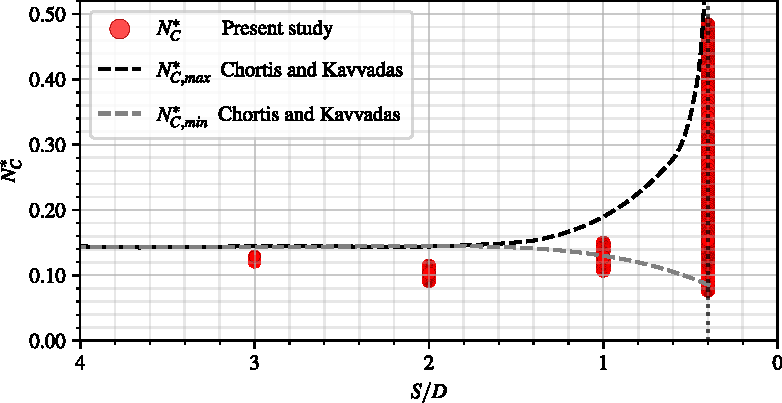
\includegraphics[scale=0.8]{Figures/Fig4.pdf}
		\vspace{12pt}
		\caption{Normalized circumferential internal force on the main tunnel at the end of construction.}
		\label{Fig4}
	\end{center}
\end{figure}
%\FloatBarrier
\vspace{8pt}

The internal forces in the tunnel lining were evaluated at the end of construction using a normalized circumferential $N_C^{\ast}=N_C/(p_0D)$ component. In Figure \ref{Fig4} (a), results near the transverse gallery were consistent with those reported by \citet{ChortisKavvadas2023}, confirming the concentration of effects in that region. Further from the gallery, lower values were observed, likely due to differences in modeling strategies, including element types, excavation procedures, and constitutive criteria.

% --------------------------------------------------------------------------
\section{Three-dimensional finite element simulations}\label{sec:results}
% --------------------------------------------------------------------------
This section presents numerical results related to the anisotropy of pressures in the twin tunnel walls, considering both elastic (EL) and viscoelastic (VEL) lining behaviors. The rock mass was modeled with an elastic modulus $E_m = 1400 \, \text{MPa}$ and Poisson's ratio $\nu_m = 0.4$. The Drucker--Prager plasticity model was adopted with cohesion $c^p = 4 \, \text{MPa}$ and friction angles $\phi^p = 0^\circ$ and $5^\circ$. Viscoplastic behavior was incorporated using a viscosity coefficient $\eta = 40{,}000 \, \text{MPa} \cdot \text{day}$, viscoplastic cohesion $c^{vp} = 2 \, \text{MPa}$, and viscoplastic friction angle $\phi^{vp} = 0^\circ$. For the concrete lining, the 28-day elastic modulus was $E_{c_{28}} = 25{,}146 \, \text{MPa}$ and Poisson's ratio $\nu_c = 0.2$.

Numerical results of lining pressures are presented at the end of construction and after 3,000 days, representing long-term viscous stabilization. The anisotropies of pressures are represented by:

\vspace{6pt}
\begin{center}
	\begin{equation}
		%\rho(\theta)=\dfrac{U(\theta)}{U(\theta=90^{\circ})} \ \text{and} 
		\chi(\theta)=\dfrac{p(\theta)}{p(\theta=90^{\circ})},
		\label{Eq9}
	\end{equation}
\end{center}
\vspace{6pt}

\noindent where $\theta$ denotes the cylindrical angle along the tunnel wall perimeter and $p(\theta)$ represents the pressure on the longitudinal tunnel lining. The values at $\theta = 90^\circ$, corresponding to the crown, are used as reference for comparison.

Two sections, S1 and S2, were adopted along the longitudinal tunnel and their locations are shown in \cref{Fig5}. Section S2 is located at the centerline of the transverse gallery, while S1 is positioned at a distance of $4R_g/3$ along the \textit{z}-axis. No results are available for $0^{\circ} < \theta < 30^{\circ}$ in S2, as this region corresponds to the gallery entrance.

\begin{figure}[!ht]
	\begin{center}
		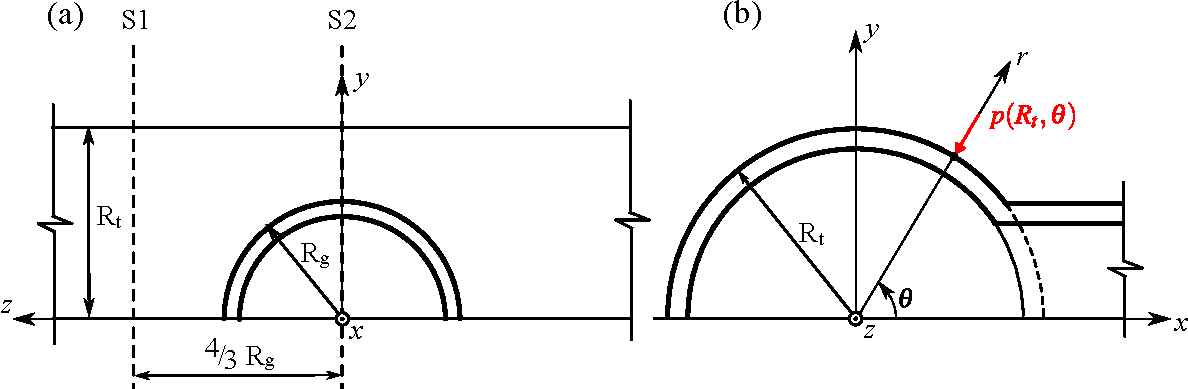
\includegraphics[scale=0.6]{Figures/Fig6.pdf}
		\vspace{12pt}
		\caption{(a) Schematic representation of the sections S1 and S2 in the longitudinal tunnel, (b) S2 and representation of pressure and displacements on the lining.}
		\label{Fig5}
	\end{center}
\end{figure}
%\FloatBarrier
\vspace{8pt}

%In \cref{Fig6}, the results show that tunnel deformations are greater at the crown ($\theta=90^{\circ}$), with the lower values at $\theta=0^{\circ} < \theta < 30^{\circ}$, indicating a predominantly horizontal ovalization. Compared to the elastic model, viscoelastic linings show higher overall convergences, about 10\% at the end of construction. In section S2, the lowest deformations occur near the gallery entrance, while for $\theta > 90^{\circ}$, the behavior becomes similar to the other section. 

%\begin{figure}[!ht]
%	\begin{center}
%		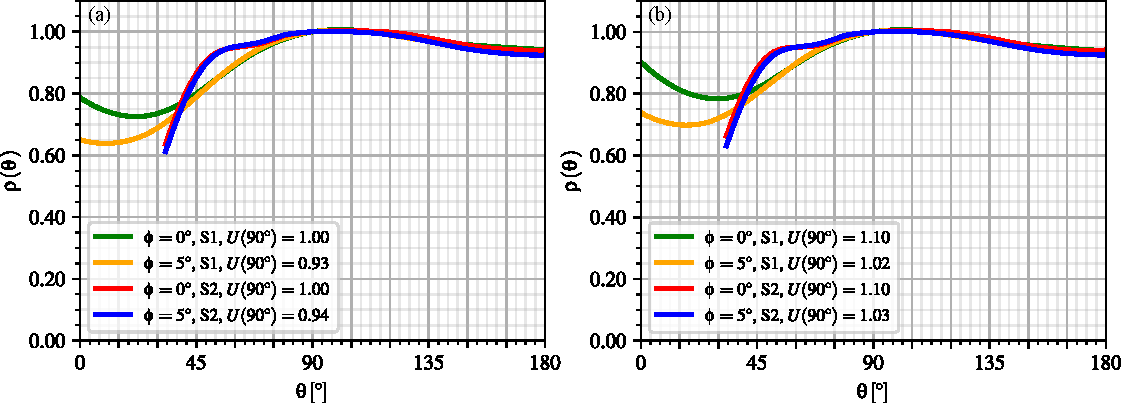
\includegraphics[scale=0.85]{Figures/rhocurto.pdf}
%		\vspace{12pt}
%		\caption{Anisotropy of deformations in longitudinal tunnel lining at the end of construction: (a) elastic lining (EL) and (b) viscoelastic lining (VEL).}
%		\label{Fig6}
%	\end{center}
%\end{figure}
%\FloatBarrier
%\vspace{8pt}

%The long-term behavior presented in \cref{Fig7} remains similar to that at the end of construction, with maximum deformations at the crown. Anisotropy decreases in the range $0^{\circ} \leq \theta \leq 45^{\circ}$, with the friction angle influencing not only the magnitude of deformations but also contributing to the anisotropic response. In section S2, despite higher convergences over time, the pattern between 30° and 75° remains consistent, suggesting minimal influence of the friction angle on anisotropy above the gallery entrance.

%\begin{figure}[!ht]
%	\begin{center}
%		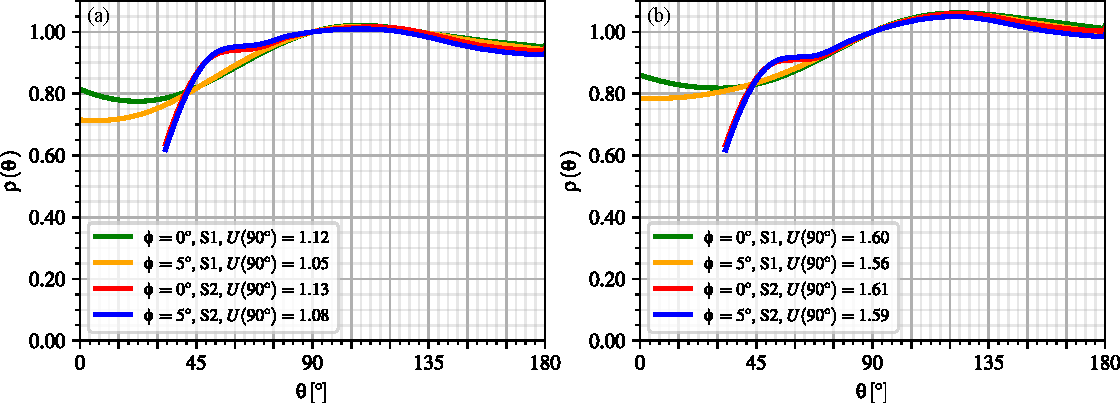
\includegraphics[scale=0.85]{Figures/rholongo.pdf}
%		\vspace{12pt}
%		\caption{Anisotropy of deformations in longitudinal tunnel lining at long-term: (a) elastic lining (EL) and (b) viscoelastic lining (VEL).}
%		\label{Fig7}
%	\end{center}
%\end{figure}
%\FloatBarrier
%\vspace{8pt}

Figure \ref{Fig8} shows that, at the end of construction, the lining pressures remain close to the reference value $p(\theta)$, except in the range $0^{\circ} < \theta < 60^{\circ}$, where a significantly increase is observed, reaching more than twice the crown pressure at $\theta = 0^{\circ}$. The friction angle influences pressure distribution, especially in section S2 at $30^{\circ} < \theta < 90^{\circ}$, where higher angles reduce pressures above the gallery entrance and amplify the contrast with the crown, reflecting greater rock mass support and lower stress transfer to the lining. 
Regarding the reference pressure $p(90^{\circ})$, higher values are observed in section S2 compared to section S1, about 14\% for $\phi=0^{\circ}$ in both elastic and viscoelastic linings, indicating that the construction of the transverse gallery significantly affects the redistribution of stresses along the tunnel at the end of construction.

\begin{figure}[!ht]
	\begin{center}
		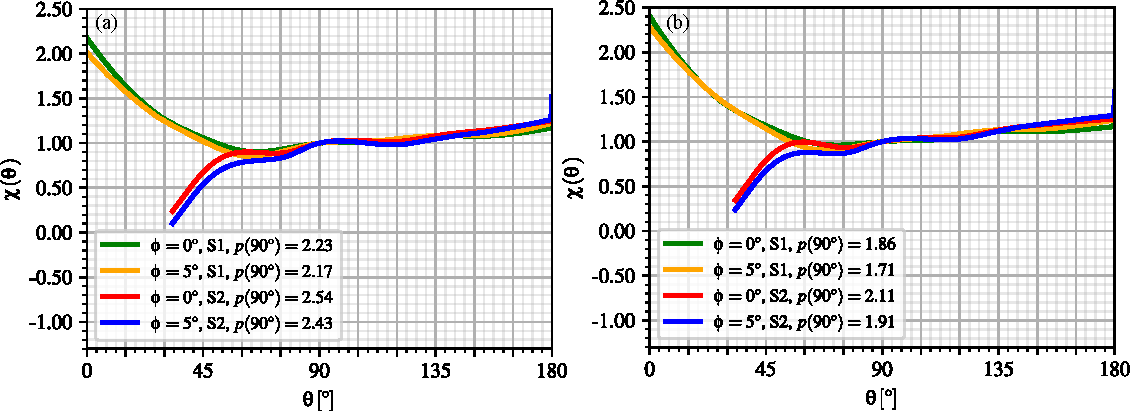
\includegraphics[scale=0.85]{Figures/chicurto.pdf}
		\vspace{12pt}
		\caption{Anisotropy of pressures in longitudinal tunnel lining at the end of construction: (a) elastic lining (EL) and (b) viscoelastic lining (VEL).}
		\label{Fig8}
	\end{center}
\end{figure}
%\FloatBarrier
\vspace{8pt}

The long-term pressures presented in \cref{Fig9} have a similar behavior to the end of construction but with increased magnitudes, and the influence of the friction angle is less pronounced. Overall, stress concentrations tend to be higher at the lateral sides of the tunnels ($\theta = 0^{\circ} \ \text{and} \ 180^{\circ}$).

In the case of elastic lining, the highest crown pressure occurs in section S2, although the increase compared to section S1 at the end of construction is relatively lower, around 6\% for a friction angle of $\phi=0^{\circ}$. In contrast, with a viscoelastic lining, the crown pressure remains nearly identical between the two sections for $\phi=0^{\circ}$, and even decreases by approximately 4\% in section S2 when $\phi = 5^{\circ}$.

\begin{figure}[!ht]
	\begin{center}
		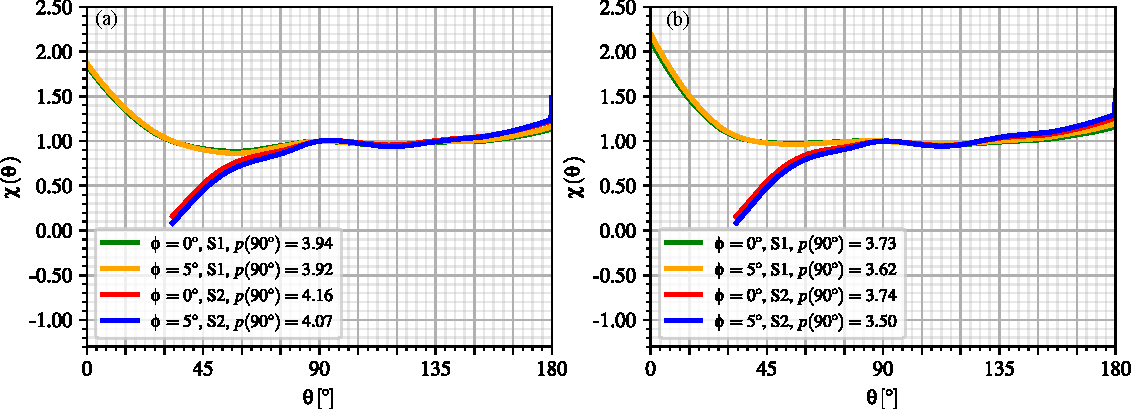
\includegraphics[scale=0.85]{Figures/chilongo.pdf}
		\vspace{12pt}
		\caption{Anisotropy of pressures in longitudinal tunnel lining at long-term: (a) elastic lining (EL) and (b) viscoelastic lining (VEL).}
		\label{Fig9}
	\end{center}
\end{figure}
%\FloatBarrier
\vspace{8pt}

% --------------------------------------------------------------------------
\section{Conclusions}\label{sec:conclusion}
% --------------------------------------------------------------------------

The computational model verification confirmed its accuracy in capturing internal forces in tunnel linings, particularly near the transverse gallery where interactions are more significant. Discrepancies in regions farther from the gallery are mainly due to differences in modeling approaches, including element types, excavation methods, and constitutive criteria.

The results obtained demonstrate the impact of constructing the transverse gallery on the redistribution of pressures along the lining of the twin tunnels. It can be observed that, at the end of construction, there is a significant increase in pressure in the lining in the lateral region adjacent to the parallel tunnel, especially in section S2, which is located on the axis of the gallery. This behavior indicates that the excavation of the transversal gallery generates a concentration of stresses above its entrance, altering the distribution. The greater angle of friction contributed to a decrease in pressures in this region.

In the long term, the pressures increase in magnitude, but the influence of the friction angle becomes less significant. Nevertheless, it is possible to observe relevant differences between the types of lining. The viscoelastic lining shows greater anisotropy in relation to the crown at $\phi=0^{\circ}$ when compared to elastic concrete. These results underscore the importance of considering the time-dependent behavior of materials and the properties of the rock mass during the design stage, particularly in critical areas such as the intersection between tunnels and galleries.

Overall, the results highlight the importance of using advanced material models and 3D analyses for the safe and realistic design of complex underground structures, especially in deep twin tunnel–gallery junctions with long-term and interactions conditions.


%-------------------------------------------------------------------------
\vspace{20pt}
\noindent \textbf{Acknowledgements.} The authors gratefully appreciate the provided by the Brazilian Research (CNPq) and the Brazilian Federal Agency for Support Evaluation of Graduate Education (CAPES).
\vspace{12pt}

%--------------------------------------------------------------------------
\noindent \textbf{Authorship statement.} The authors hereby confirm that they are the sole liable persons responsible for the authorship of this work, and that all material that has been herein included as part of the present paper is either the property (and authorship) of the authors, or has the permission of the owners to be included here.

\bibliography{bibliography}

\end{document}